\documentclass[11pt,letterpaper,twocolumn]{article}
\usepackage[utf8]{inputenc}
\usepackage[spanish]{babel}
\usepackage{amsmath}
\usepackage{amsfonts}
\usepackage{amssymb}
\usepackage{float}
\usepackage{graphicx}
\usepackage{subfigure}
\usepackage{listings}
\usepackage[left=2cm,right=2cm,top=2cm,bottom=2cm]{geometry}
\begin{document}
\title{\huge{\textbf{
Análisis del perfil de un haz láser gaussiano en MATLAB\\Profile analysis of a Gaussian laser beam in MATLAB}}}
\author{\small \textit{M. Sabogal $^{1}$}\\
	\small \textit{ $^{1}$ Estudiante del programa de Física, Universidad del Atlántico, Barranquilla-Colombia}}
\date{} 

\twocolumn[
\begin{@twocolumnfalse}
\maketitle
\begin{center}
{\rule[0mm]{160mm}{0.2mm}}
\end{center}
\begin{abstract}
\textit{Se realizo el estudio y análisis de la imagen del perfil de un haz láser gaussiano, en dos diferentes escalas de colores, RGB y grises, utilizando las herramientas computacionales de MATLAB, a partir de las cuales se determinaron algunas propiedades del haz, como su distribución de intensidades, ancho en el FWHM, $1/e$ y $1/e^{2}$ , su cintura, y los porcentajes de energía concentrada para cada una de las regiones con valores de intensidad superiores o iguales a los puntos FWHM, $1/e$ y $1/e^{2}$, tanto unidimensionalmente cómo bidimensionalmente.\\
\\
\textbf{Palabras claves: Perfil, gaussiano,FWHM.}}
\begin{center}
\textbf{Abstract} 
\end{center}
\par 
\textit{it was carried out the study and analysis of the profile image of a Gaussian laser beam, in two different color scales, RGB and gray, using the MATLAB computational tools, from which some beam properties were determined, as well as their distribution of intensities, width in the FWHM, $ 1/e $ and $1/e^{2}$, his waist, and the percentages of concentrated energy for each of the regions with intensity values greater than or equal to the FWHM points, $1/e$ and $1/e^{2}$, both one-dimensionally and two-dimensionally.\\
\\
\textbf{Keywords: Profile, Gaussian, FWHM.}}
\end{abstract}
\begin{center}
{\rule[0mm]{160mm}{0.2mm}}
\end{center}
\end{@twocolumnfalse}
]

\section*{\normalsize{INTRODUCCIÓN}} 
La tecnología láser es una de las  áreas de las modernas tecnologías que mayor desarrollo ha tenido. Cuando se inventó el láser, en 1960, se consideró que era una solución en busca de un problema, y hoy la tecnología láser se aplica en áreas muy diferentes, tales como : medicina, comunicación, dispositivos de uso cotidiano, militar y en la  industria. El láser (light amplification by stimulated emission of radiation, por sus siglas en ingles) es un dispositivo que utiliza un efecto de la mecánica cuántica, la emisión inducida o estimulada, para generar un haz de luz coherente tanto espacial como temporalmente. La coherencia espacial se corresponde con la capacidad de un haz para permanecer con un pequeño tamaño al transmitirse por el vacío en largas distancias y la coherencia temporal se relaciona con la capacidad para concentrar la emisión en un rango espectral muy estrecho.\\
\par 
La radiación láser se utiliza en el sentido más amplio para incluir todo el espectro electromagnético. El láser actual abarca el rango de longitud de onda de aproximadamente 200 $nm$ a 400 $\mu m$, desde la generación del primer rayo láser en 1960, las técnicas de detección se desarrollan para reconocer y analizar el rayo descubierto. En general, el análisis del rayo láser se basa en la medición de energía, la distribución de intensidad del rayo láser, la divergencia del rayo, el parámetro de cintura y el número de modos, entre otros$^{[1]}$. Se desea estudiar algunas de las propiedades de un láser antes mencionadas, cómo su distribución de intensidad, a partir del análisis de imágenes en MATLAB a una fotografía experimental del perfil de un láser. 
\subsection*{Haz Gassuiano}
En las últimas décadas, el uso de rayos láser se ha generalizado. Los láseres se utilizan tanto en la ciencia como en la tecnología, desde el análisis espectroscópico hasta la lectura de códigos de barras. Los rayos láser de distintos tipos y colores tienen algunas características en común: están compuestos por una banda estrecha de longitudes de onda, al punto que podemos llamarlos "monocromáticos" (de una sola longitud de onda), y están colimados, es decir, La energía luminosa está restringida en la dirección transversal a la dirección de propagación para formar un haz estrecho. En un plano que es transversal a la dirección de propagación, la intensidad del haz disminuye en una forma gaussiana típica.$^{[2]}$\\
\par 
Las ondas más simples son la onda plana, que tiene la forma $\cos(kx-wt)$, y la onda esférica, que tiene la forma $\cos(kR-wt)/R$. Estos son modelos útiles. El haz gaussiano ( ecuación \ref{1}) es el modelo más simple de un haz dirigido que satisface las ecuaciones de Maxwell y la ecuación de onda, al menos en la aproximación paraxial. También resulta que las salidas de los resonadores de espejo esférico y los láseres son a menudo rayos gaussianos. El haz de Gaussiano es igual que el paquete de ondas gaussiano en la mecánica cuántica, siendo lo suficientemente complejo como para ser interesante, pero lo suficientemente simple para ser manejable.$^{[3]}$

\begin{equation}
E^{(+)}(r)=E_{o}^{(+)} \dfrac{\omega_{o}}{\omega (z)} e^{\dfrac{-r^{2}}{\omega^{2}(z)}} e^{ikz-i\tan^{-1}(\dfrac{z}{z_{o}})} e^{ik\dfrac{r^{2}}{2R(z)}}
\label{1}
\end{equation}
\par 
Este es el haz Gaussiano o TEM$_{0,0}$ (para “Modo transversal electromagnético”, como para la onda plana; el subíndice proviene de la jerarquía de haces de Hermite-Gauss, donde TEM$_{0,0}$ es el modo fundamental). En esta expresión, se encuentra en coordenadas polares $(r,z)$ con $r=\sqrt{x^2 + y^2}$; $E_{o}$ es, como siempre, una constante de amplitud de campo general; $z_{o}$ es una constante llamada longitud de Rayleigh (o "rango de Rayleigh") y $\omega_{o}$ es el parámetro de la cintura del haz o el radio del haz, estos dos últimos presentan la ultima relación: 
$$z_{o}=\dfrac{\pi \omega_{o}^{2}}{\lambda}$$
\par 
Si $R$ es el radio de curvatura de los frentes de onda, y $\omega$ es la cintura del haz o Spot en función de $z$, de la forma:
$$\omega(z)=\omega_{o}\sqrt{1+(\dfrac{z}{z_{o}})^{2}}$$
$$R(z)=z(1+(\dfrac{z}{z_{o}})^{2})$$
\subsection*{Perfil de intensidad}
El primer factor en la ecuación \ref{1} es el factor de amplitud, que describe completamente el perfil de intensidad del haz gaussiano. En este sentido, este es el factor más útil para comprender el comportamiento del haz gaussiano. La intensidad es solo el módulo cuadrado de la ecuación 1, pero los otros dos factores no contribuyen:
\begin{equation}
I(r,z)=I_{o}[\dfrac{\omega_{o}}{\omega (z)}]^{2} e^{\dfrac{-2r^{2}}{\omega^{2}(z)}}
\end{equation}
\par 
Se ha definido $I_{o}= 2|E_{o}^{(+)}|^{2}$ como la intensidad máxima del haz gaussiano (que ocurre en el centro $r=0$). Claramente, la intensidad cae en la dirección radial como una función gaussiana, de ahí el nombre "rayo gaussiano". Además, tenga en cuenta que $\omega(z)$ es una medida del ancho del gaussiano y se reduce al valor mínimo $\omega_{o}$ en $z=0$. Tomando ésto en consideración, si se realiza un analisis en $z=0$, se obtiene: 
\begin{equation}
I(r)=I(r,0)=I_{o} e^{\dfrac{-2r^{2}}{\omega_{o}^{2}}}
\label{inten}
\end{equation}
\par 
Que representa la distribucion de intensidades en el spot que se puede apreciar en la figura, donde el radio de curvatura es cero.
\begin{figure}[h!]
\begin{center}
\includegraphics[scale=0.4]{spot.png}
\caption{Cintura de un haz, cuando $z=0$.$^{[5]}$}
\end{center}
\end{figure}
\subsection*{Modos transversales electromacneticos}
Como la luz está compuesta de ondas electromagnéticas, las leyes que gobiernan los campos eléctricos y magnéticos en las cavidades reflectoras controlan la distribución espacial de la luz láser que resuena dentro de una cavidad láser. Cada distribución permitida de un campo electromagnético a través del eje largo del resonador se denomina modo electromagnético transversal (TEM). Un láser puede operar en uno o varios TEM al mismo tiempo. Muchos láseres están diseñados para funcionar en el modo TEM. En este modo, la viga tiene una sección transversal circular con una intensidad máxima en el centro y una intensidad decreciente en el punto radial eliminado del centro. El modo TEM produce el rayo láser de menor divergencia y de menor diámetro. La operación multimodo aumenta la potencia de salida pero disminuye la coherencia y aumenta la divergencia.$^{[1]}$\\
\begin{figure}[h!]
\begin{center}
\includegraphics[scale=0.25]{tem.png}
\caption{Varios TEM modos con el mismo $\omega_{o}$, y normalizadas para que tengan el mismo poder optico.$^{[5]}$}
\end{center}
\end{figure}
\par 
El modo TEM$_{00}$ fundamental es solo uno de los muchos modos transversales que satisfacen los criterios de propagación de ida y vuelta descritos en la propagación del haz gaussiano. La Figura se muestra ejemplos de las inensidades de soluciones primarias de orden inferior de Hermite-Gauss (rectangulares) a la ecuación de propagación. Tenga en cuenta que los subíndices n y m en el modo propio TEM nm se correlacionan con el número de nodos en las direcciones x e y. En cada caso, los lóbulos adyacentes del modo están desfasados 180 grados.$^{[4]}$
\section*{-Implementación, interpretación física y resultados}
Con el fin de estudiar propiedades de un haz láser, cómo su distribución de intensidad y la cintura del haz, entre otras; se realizo un análisis a la imagen del perfil de un haz láser (figura $3$), mediante las herramientas computacionales de MATLAB.\\
\begin{figure}[h!]
\begin{center}
\includegraphics[scale=0.15]{green-laser-2.JPG}
\caption{Imagen de analisis, del perfil de un haz laser.}
\end{center}
\label{ima}
\end{figure}
\par 
Utilizando la función \textit{imread()} de MATLAB, se tomo la imagen de análisis \ref{ima} y se obtuvo su representación o descomposición en la escala de colores RGB, y mediante la función \textit{imagesc()} se visualizo la intensidad para cada una de las descomposiciones o canales (rojo, verde y azul), cómo se visualiza en la figura, en la que se observa que el modo transversal electromagnético del haz de estudio, es el fundamental, es decir TEM$_{0,0}$:
\begin{figure}[h!]
\begin{center}
\subfigure[rojo] {\includegraphics[scale=0.527]{rojo.eps}}\\
\subfigure[verde] {\includegraphics[scale=0.527]{verde.eps}}\\
\subfigure[azul] {\includegraphics[scale=0.527]{azul.eps}}
\caption{Descomposición de la imagen de analisis en RGB.}
\end{center}
\label{ima}
\end{figure}
\par 
Es de apreciar que la mayor parte de la intensidad de la imagen original se encuentra en la representación verde, a partir de la cual se realizara el análisis. Se tomaron los datos referentes al verde, y mediante las funciones \textit{max()} y \textit{ind2Sub()} se determino el máximo y su posición en la matriz de intensidades (del verde).\\
\par 
Posteriormente se convirtiendo los datos del formato \textbf{uint8} a números reales mediante la función \textit{double()}, y se normalizo la matriz de intensidades referente al verde, dividiendo cada uno de sus elementos entre el máximo encontrado. Tomando la fila o columna en la que se encuentra el máximo, y graficando ésta en función ya sea de x o y, se observa la distribución unidimensional que presenta el haz láser a lo largo de ese eje (normalizado), cómo se observa en la figura $5$: 
\begin{figure}[h!]
\begin{center}
\subfigure[a=0.9952, b=0.4999, c=0.1624] {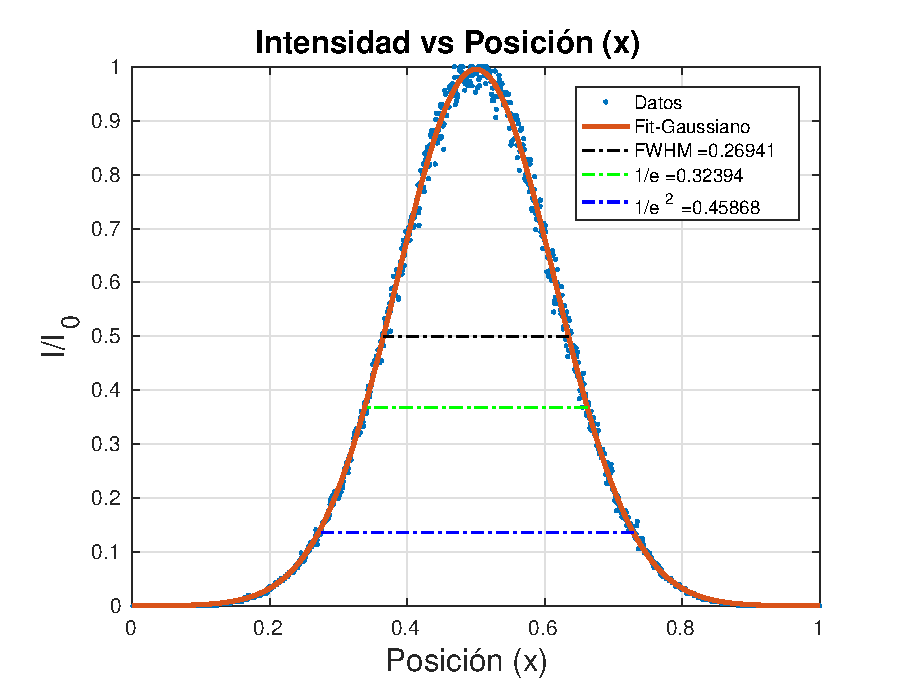
\includegraphics[scale=0.6]{dis-rgb-x.eps}}
\subfigure[a=0.9595, b=0.5001, c=0.1970] {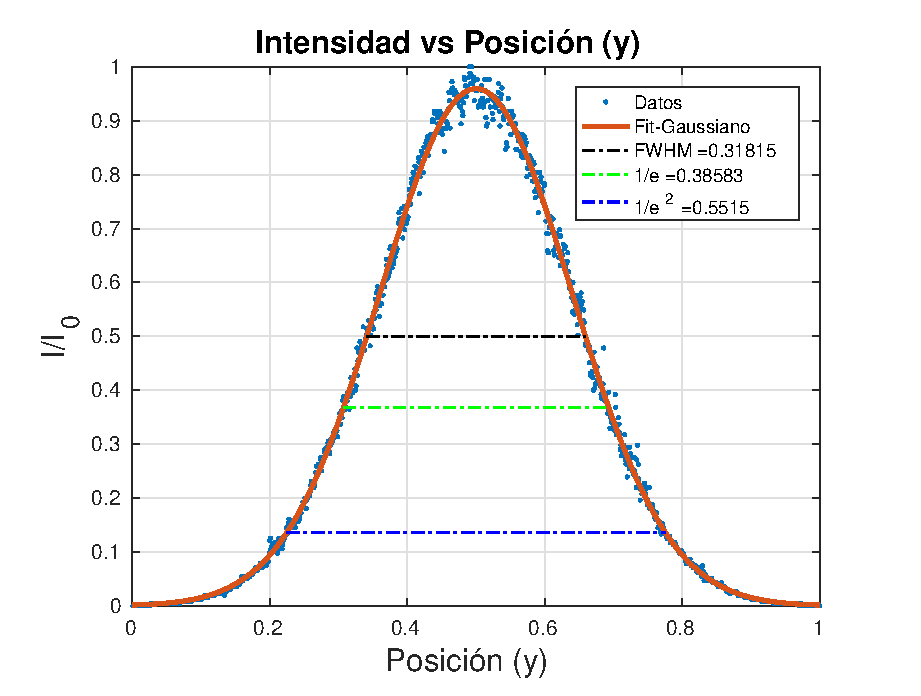
\includegraphics[scale=0.6]{dis-rgb-y.eps}}
\caption{Distribuciones unidimensionales de intensidades.}
\end{center}
\label{distribuciones1D}
\end{figure}
\par 
Utilizando la función \textit{lsqcurvefit()} y modelando una función de fiteo según la ecuación \ref{fit}, la cual concuerda con la distribución de intensidades de la ecuación \ref{inten}, se realizo un fitting a la distribución unidimensional de intensidades encontrada en la figura $5$.\\

\begin{equation}
y=f(x)=a e^{- \dfrac{(x-b)^{2}}{c^{2}}}
\label{fit}
\end{equation}
\\
\par 
Al tener los valores de las constantes de la función de fitting, se obtuvo la ecuación inversa (\ref{inversa}) la cual permite encontrar los dos valores de $x$ que generan un $f(x)$ especifico, a partir de éstos valores fue posible determinar los anchos para el FWHM, 1/e y 1/e$^{2}$, presentes en la figura, donde el valor encontrado para $y=1/e^{2}$ corresponde a $\omega_{o}$, es decir la cintura del haz.\\
\begin{equation}
x=b \pm c \sqrt{\ln(\dfrac{a}{y})}
\label{inversa}
\end{equation}

\begin{figure}[h!]
\begin{center}
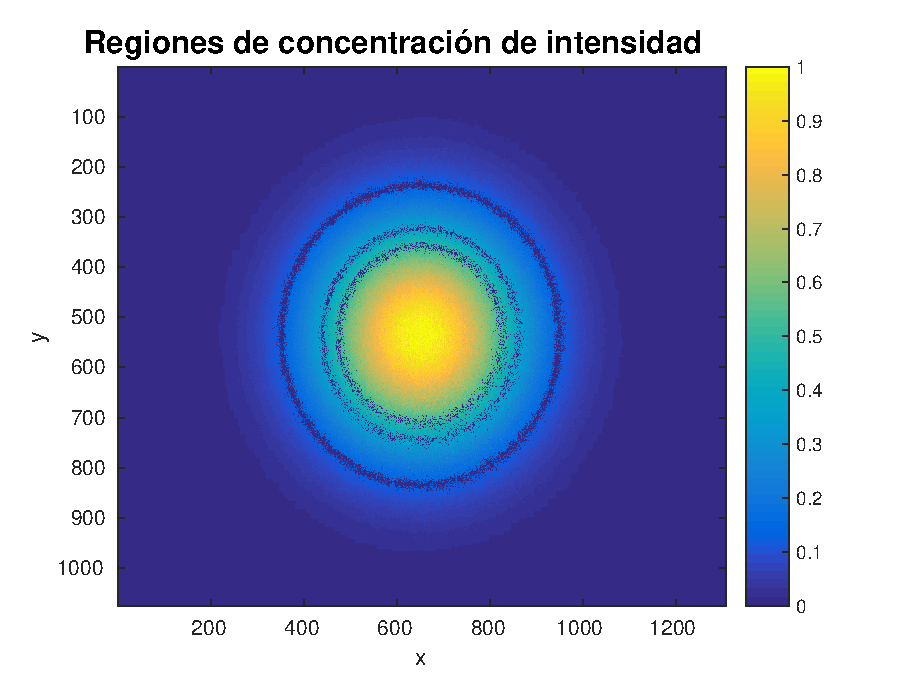
\includegraphics[scale=0.6]{anillos.eps}
\caption{Regiones de concentrarion, anillo interior (FWHM), anillo medio ($1/e$) y anillo mayor ($1/e^{2}$)}
\end{center}
\label{anillos}
\end{figure}
\par 
Posteriormente, con el fin de determinar el porcentaje de intensidad (es decir energía) presente en las regiones (círculos) de la figura $6$ se sumaron los valores de intensidad iguales o mayores a los puntos FWHM ($I \geq 0.5$, circulo interno), 1/e ($I \geq 1/e$, circulo medio) y 1/e$^{2}$ ($I \geq 1/e^{2}$, circulo de mayor diámetro), y se ponderaron con respecto a la intensidad total, tanto de manera unidimensional cómo bidimensional, obteniendo las siguientes proporciones:\\  
\begin{figure}[h!]
\begin{center}
\subfigure[1-D] {\includegraphics[scale=0.6]{int-1d-rgb.eps}}
\subfigure[2-D] {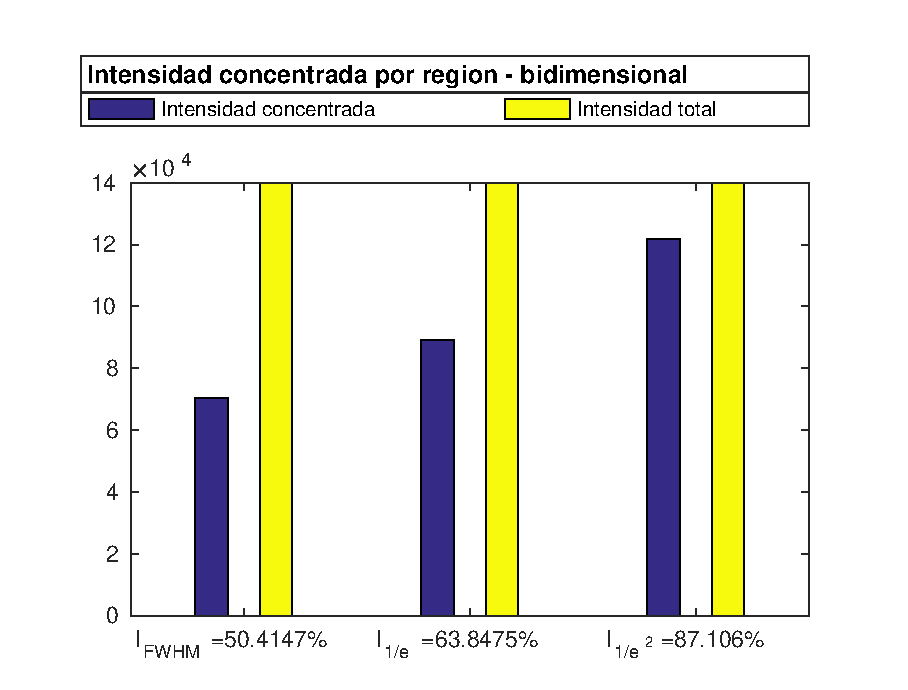
\includegraphics[scale=0.6]{int-2d-rgb.eps}}
\caption{Porcentaje de intensidades por region en RGB}
\end{center}
\end{figure}
\par 
Es de apreciar que el porcentaje de energía presente para cada región, es menor en su forma bidimensional que en la unidimensional, sin embargo, ambos resultados concuerdan con los obtenidos al integrar una función (Gaussiana) analítica normalizada, en especial el porcentaje de energía presente en la region con un radio de $1/e^{2}$, la cual se encuentra $\sim 13 \%$ por debajo de la intensidad total, concordando con la literatura con respecto al tema $^[1]$.
\par 
Con el propósito de comparar y verificar los datos obtenidos anteriormente, se realizo el análisis general de la figura \ref{1} en escala de grises, mediante las funciones \textit{imread()} y \textit{rgb2gray()} de MATLAB, de la cual solo se obtiene una matriz de intensidades, a diferencia que en el caso de la escala de RGB donde se obtienen tres. Utilizando nuevamente la función \textit{imagesc()}, se visualiza en la figura la intensidad en el plano ($x,y$):\\   
\begin{figure}[h!]
\begin{center}
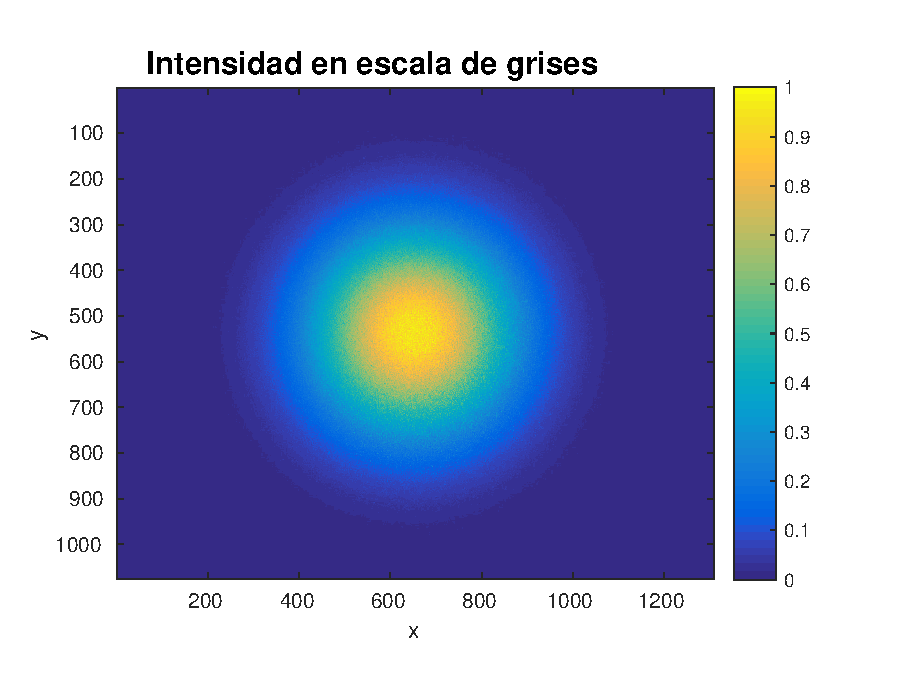
\includegraphics[scale=0.6]{gris.eps}
\caption{Descomposicion de la imagen de analisis en escala de grises}
\end{center}
\end{figure}
\par 
De manera similar al análisis en RGB, se obtuvo la distribución unidimensional de intensidades a lo largo del eje $x$ en éste caso, y se realizo el fitting respectivo modelado por la función \ref{fit}, cómo se observa en la figura \ref{dis-1D-gris}.\\ 

\begin{figure}[h!]
\begin{center}
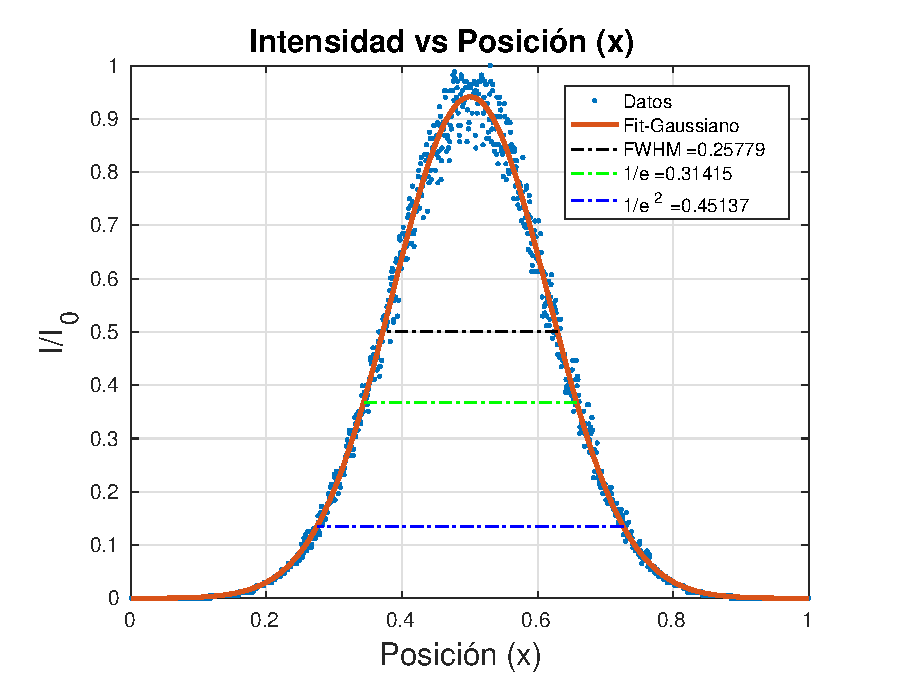
\includegraphics[scale=0.6]{dis-1d-gris.eps}
\caption{Distribucion unidiemnsional de intensidades en escaal de grises; a=0.9413, b=0.5005, c=0.1621}
\end{center}
\label{dis-1D-gris}
\end{figure}
\par 
Posteriormente se determinaron los porcentajes de intensidad (energía) para las regiones con respecto al FWHM,$1/e$ y $1/e^{2}$ para el análisis de la imagen en escala de grises, tanto de manera unidimensional ćomo bidimensional, como se observa en la figura:\\ 
\begin{figure}[h!]
\begin{center}
\subfigure[1-D] {\includegraphics[scale=0.6]{int-1d-gris.eps}}
\subfigure[2-D] {\includegraphics[scale=0.6]{int-2d-gris.eps}}
\caption{Porcentaje de intensidades por region en escala de grises}
\end{center}
\end{figure}
\par 
Se aprecia que los resultados del análisis de en escalas de grises son muy cercanos en a los resultados del análisis en RGB, ésto es debido  a que la intensidad perdida en los canales de rojo y azul, es algunos ordenes de magnitud menor que la intensidad del canal verde.
\section*{\normalsize{CONCLUSIÓN}}
Mediante las herramientas computacionales de MATLAB, se pudo estudiar y analizar la imagen del perfil de un haz, en las escalas de colores RGB y grises, en ambas se encontraron sus distribuciones de intensidad tanto unidimensional cómo bidimensional, resultado todas gaussianas y en su modo fundamental TEM$_{0,0}$, lo cual concuerda con los resultados analíticos, de manera similar y apartir de estos hechos, se determinaron los anchos de los puntos FWHM, $1/e$ y $1/e^{2}$ en todas las distribuciones unidimensionales de la intensidad, y por ende la cintura del haz en cuestión, también se determinaron los porcentajes de intensidad (enegria) para cada una de las regiones con valores de intensidad superiores o iguales a los puntos FWHM, $1/e$ y $1/e^{2}$, tanto unidimensionalmente cómo bidimensionalmente, encontrando que los datos obtenidos en el análisis en RGB, tomando solo el canal verde, coinciden o se aproximan a los determinados en el análisis en escala de grises, donde la intensidad concentrada en la región correspondiente al FHWM es de $\sim 75\%$ unidimensional y $\sim 50\%$ bidimensionalmente, para $1/e$, $\sim 83\%$ y $\sim 62\%$, y  finalmente para $1/e^{2}$, $\sim 95 \%$ y $\sim 87 \%$, respectivamente.  
\section*{Referencias} 
\begin{itemize} 
\item[[ 1]] Yas A. Alsultanny. Laser Beam Analysis Using Image Processing. Journal of Computer Science 2, 2006. 
\item[[ 2]] Enrique J. Galvez. Gaussian Beams. Department of Physics and Astronomy Colgate University, 2009.

\item[[ 3]] Daniel A. Steck. Classical and Modern Optics. Oregon Center for Optics and Department of Physics, University of Oregon, 2006.

\item[[ 4]] Gaussian Beam Optics- CVI Melles Griot 2009 Technical Guide, vol 2, issue 1.

\item[[ 5]]Gary Eden ,Tom Galvin. Optical Resonator Modes ,ECE 455 Optical Electronics. ECE Illinois. 
\end{itemize}
\subsection*{Anexos}
\begin{lstlisting}
1. Codigo en MATLAB para el 
analisis de imagen en RGB:

% Lectura de la imagen
A=imread('~/Documentos/laser2.JPG'); 

% Asignacion de cada canal
Cr=double(A(:,:,1)); 
Cg=double(A(:,:,2));
Cb=double(A(:,:,3));

% Posicion del maximo
[Max,b]=max(Cg(:)); 
[n_max, m_max] = ind2sub(size(Cg),b); 

% Asignacion de variables 1-D
 para el fitting, y normalizacion
 
data_1D=Cg(n_max,:)/Max ; 
dominio=[1:1:length(data_1D)];   
dominio=dominio/length(dominio);
 
% Intensidad total 
I_total_1D=sum(data_1D);

% Puntos de interes
fwhm=(1/2); e_1=(1/exp(1));
e_2=(1/exp(2));   

% Intensidad en el FWHM-1D
I_fwhm_1D=sum(data_1D.*(data_1D>=fwhm)); 
I_fwhm_porcentual_1D 
 =I_fwhm_1D/I_total_1D*100; 
 
% Intensidad en el 1/e-1D
I_exp1_1D=sum(data_1D.*(data_1D>=e_1));
I_exp1_porcentual_1D
 =I_exp1_1D/I_total_1D*100;  
 
% Intensidad en el 1/e^{2}-1D 
I_exp2_1D=sum(data_1D.*(data_1D>=e_2)); 
I_exp2_porcentual_1D
 =I_exp2_1D/I_total_1D*100;  

% Asignacion de variables 2-D
 para el fitting, y normalizacion
 
data_2D=Cg/Max; 
I_total_2D=sum(sum(data_2D));   

% Intensidad en el FWHM-2D
I_fwhm_2D=sum(sum(data_2D.*(
data_2D>=fwhm)));

I_fwhm_porcentual_2D
 =I_fwhm_2D/I_total_2D*100; 

% Intensidad en el 1/e-2D
I_exp1_2D=sum(sum(data_2D.*(
data_2D>=e_1)));
I_exp1_porcentual_2D
 =I_exp1_2D/I_total_2D*100;

% Intensidad en el 1/e^{2}-2D
I_exp2_2D=sum(sum(data_2D.*(
data_2D>=e_2))); 
I_exp2_porcentual_2D
 =I_exp2_2D/I_total_2D*100; 

% Fitting
[Cnts,ince]=lsqcurvefit(@myfun1,
[1,3,27],dominio,data_1D); 

% Determinacion de los anchos 
 para cada punto
 
Ancho_fwhm=Ancho(Cnts,fwhm); 
Ancho_e1=Ancho(Cnts,e_1);  
Ancho_e2=Ancho(Cnts,e_2);

% funciones utilizadas

function f=myfun1(a,x)
f=a(1)*exp(-((x-a(2))/a(3)).^2); 
end

function f=Ancho(Cnts,punto)
x2=Cnts(2)+
Cnts(3)*sqrt(log(Cnts(1)/punto));
 
x1=Cnts(2)-
Cnts(3)*sqrt(log(Cnts(1)/punto));
 
f=[x1,x2,abs(x2-x1)]; 
end  


2. Codigo en MATLAB para el analisis 
de imagen en escala de Grises:

% Lectura de la imagen
A=imread('~/Documentos/laser2.JPG'); 

% imagen en escala de grises
B=double(rgb2gray(A));

% Posicion del maximo
[Max,b]=max(B(:)); 
[n_max, m_max] = ind2sub(size(B),b); 

% Asignacion de variables 1-D
 para el fitting, y normalizacion
 
data_1D=B(n_max,:)/Max ; 
dominio=[1:1:length(data_1D)];   
dominio=dominio/length(dominio);
 
% Intensidad total 
I_total_1D=sum(data_1D);

% Puntos de interes
fwhm=(1/2); e_1=(1/exp(1));
e_2=(1/exp(2));   

% Intensidad en el FWHM-1D
I_fwhm_1D=sum(data_1D.*(
data_1D>=fwhm)); 
I_fwhm_porcentual_1D 
 =I_fwhm_1D/I_total_1D*100; 
 
% Intensidad en el 1/e-1D
I_exp1_1D=sum(data_1D.*(
data_1D>=e_1));
I_exp1_porcentual_1D
 =I_exp1_1D/I_total_1D*100;  
 
% Intensidad en el 1/e^{2}-1D 
I_exp2_1D=sum(data_1D.*(
data_1D>=e_2)); 
I_exp2_porcentual_1D
 =I_exp2_1D/I_total_1D*100;  

% Asignacion de variables 2-D
 para el fitting, y normalizacion
 
data_2D=Cg/Max; 
I_total_2D=sum(sum(data_2D));   

% Intensidad en el FWHM-2D
I_fwhm_2D=sum(sum(data_2D.*(data_2D>=fwhm)));
I_fwhm_porcentual_2D
 =I_fwhm_2D/I_total_2D*100; 

% Intensidad en el 1/e-2D
I_exp1_2D=sum(sum(data_2D.*(data_2D>=e_1)));
I_exp1_porcentual_2D
 =I_exp1_2D/I_total_2D*100;

% Intensidad en el 1/e^{2}-2D
I_exp2_2D=sum(sum(data_2D.*(data_2D>=e_2))); 
I_exp2_porcentual_2D
 =I_exp2_2D/I_total_2D*100; 

% Fitting
[Cnts,ince]=lsqcurvefit(@myfun1,
[1,3,27],dominio,data_1D); 

% Determinacion de los anchos 
 para cada punto
 
Ancho_fwhm=Ancho(Cnts,fwhm); 
Ancho_e1=Ancho(Cnts,e_1);  
Ancho_e2=Ancho(Cnts,e_2);

\end{lstlisting}
\end{document}
